\paragraph{В четвертой} главе приводится имитационное моделирование развиваемых алгоритмов. В качестве алгоритма
для сравнения используется параллельный коррелятор с алгоритмом уточнения частоты.

\begin{figure}[H]
\center\scalebox{1}{\includegraphics[width=1\linewidth]{modeling_general.eps}}
	\caption{Схема эксперимента}
	\label{pic:ar_dma_probability}
\end{figure}

\underline{Алгоритм} оценки параметров сигнала с расширенным спектром на фоне аддитивного белого шума.
График вероятности оценки частоты в допустимом диапазоне входной расстройки представлен на рисунке
\ref{pic:lpc_for_1_probability}. Моделирование проводилось с аддитивным шумом, заданным в полосе от 0 Гц до
половины частоты дискретизации для одного, двух и трех шагов уточнения АКФ.
\begin{figure}[H]
\center\scalebox{1}{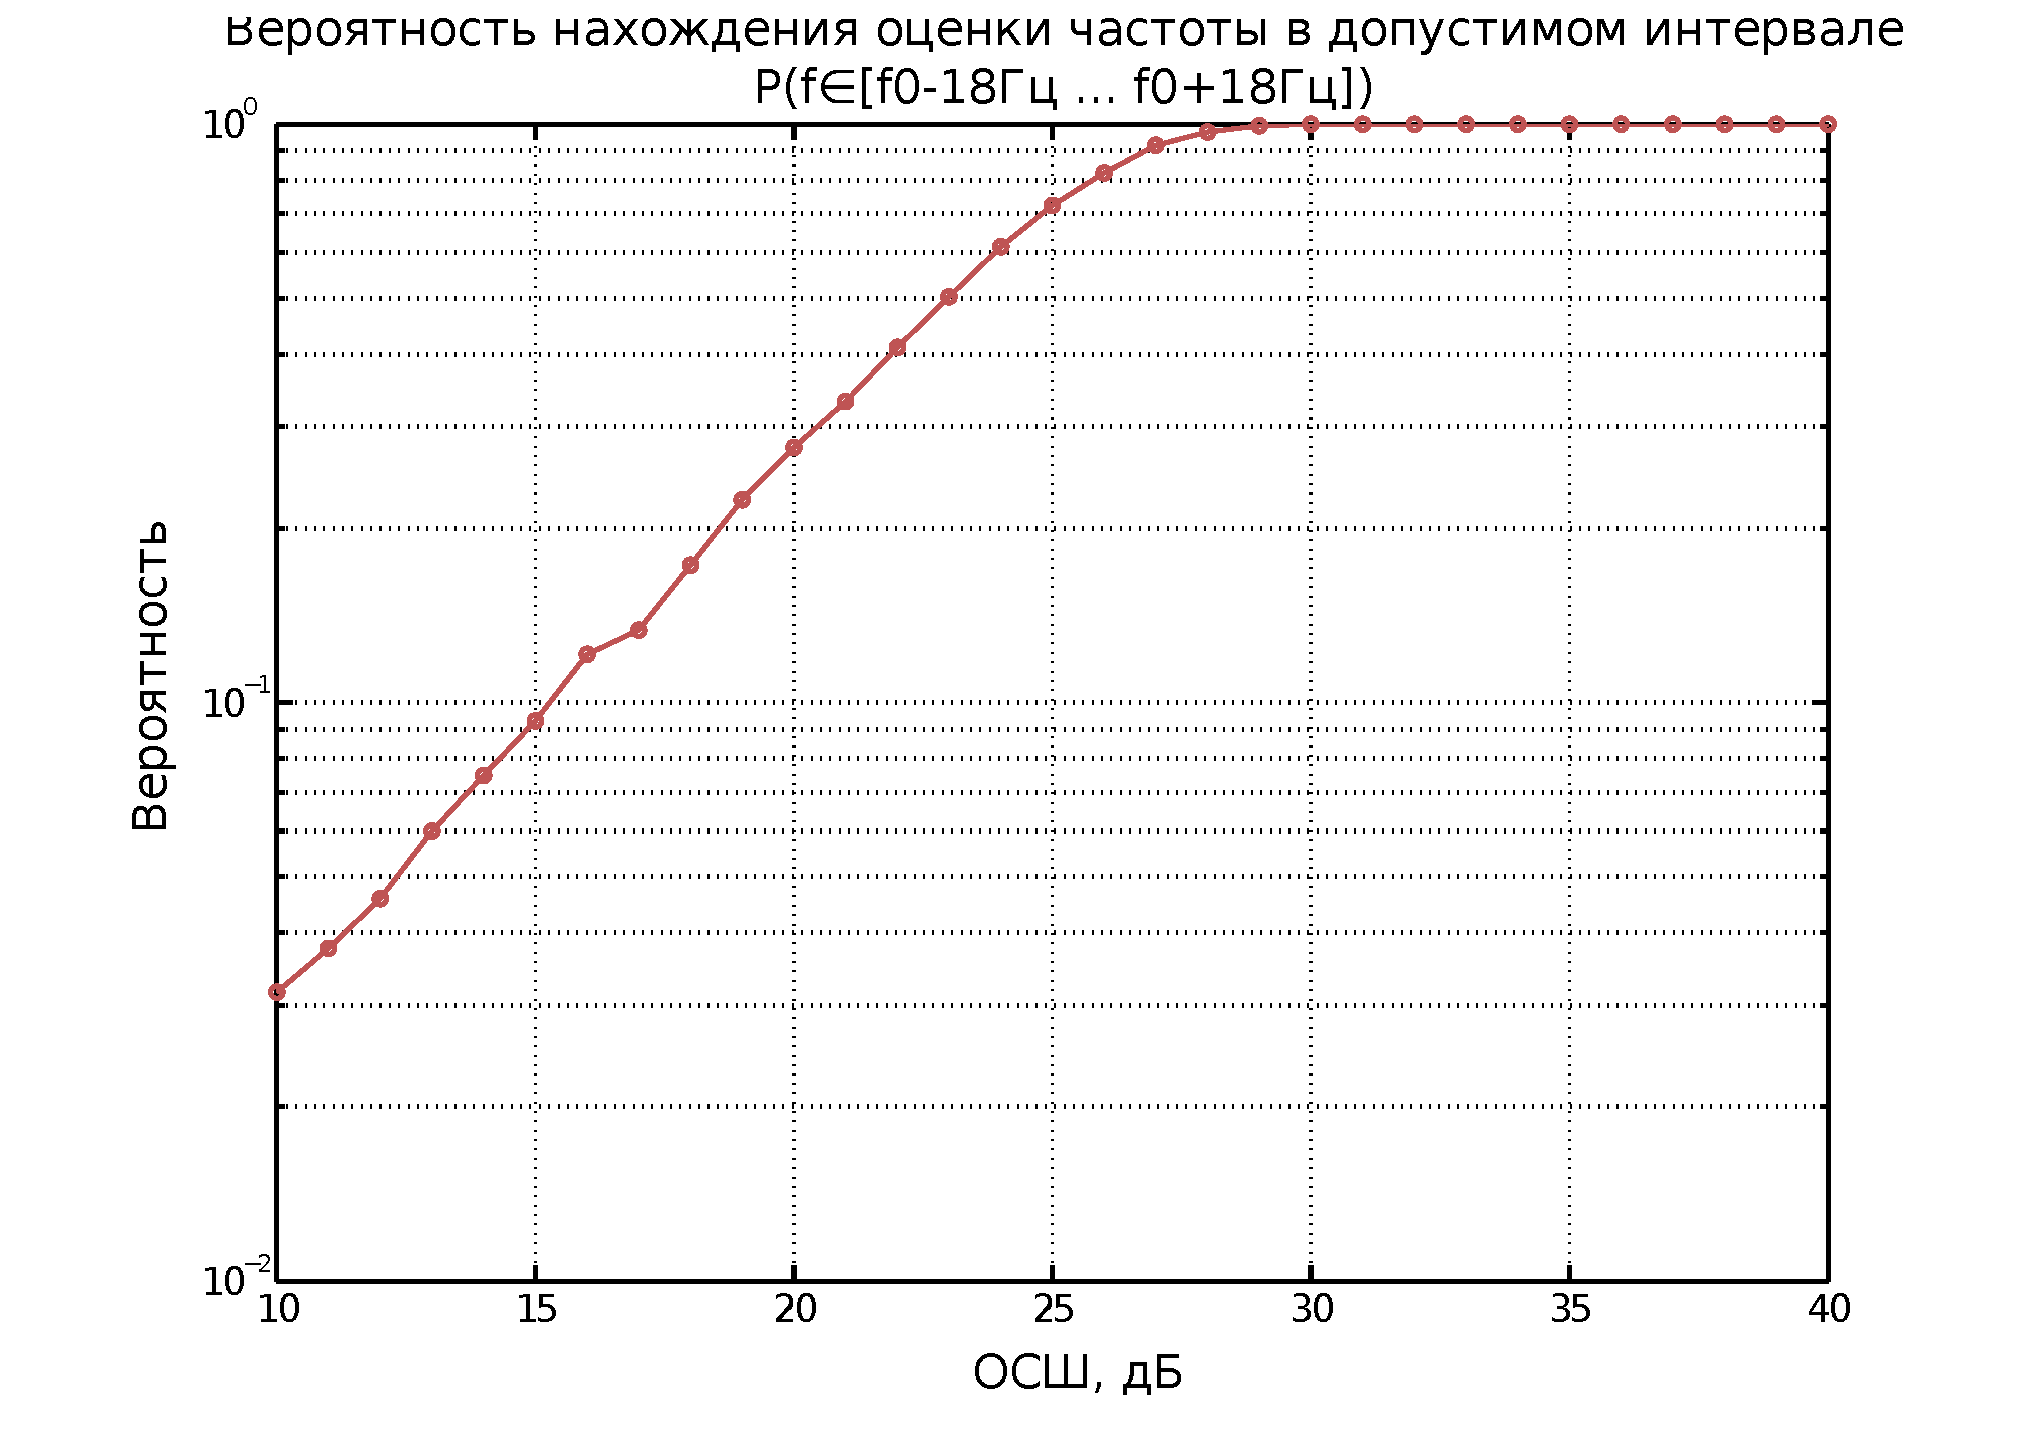
\includegraphics[width=1\linewidth]{lpc_for_1_probability.eps}}
	\caption{Вероятность оценки частоты удовлетворяющей допустимой входной расстройке}
	\label{pic:lpc_for_1_probability}
\end{figure}

%%%%%%%%%
\underline{Алгоритм} оценки параметров ШПС в условиях интерференции
(Delay and Multiply Approach + уточненный АР).

График вероятности оценки частоты в допустимом диапазоне входной расстройки представлен на рисунке
\ref{pic:ar_dma_probability}. Моделирование проводилось с аддитивным шумом, заданным в полосе от 0 Гц до
половины частоты дискретизации для одного, двух и трех шагов уточнения АКФ.
\begin{figure}[H]
\center\scalebox{1}{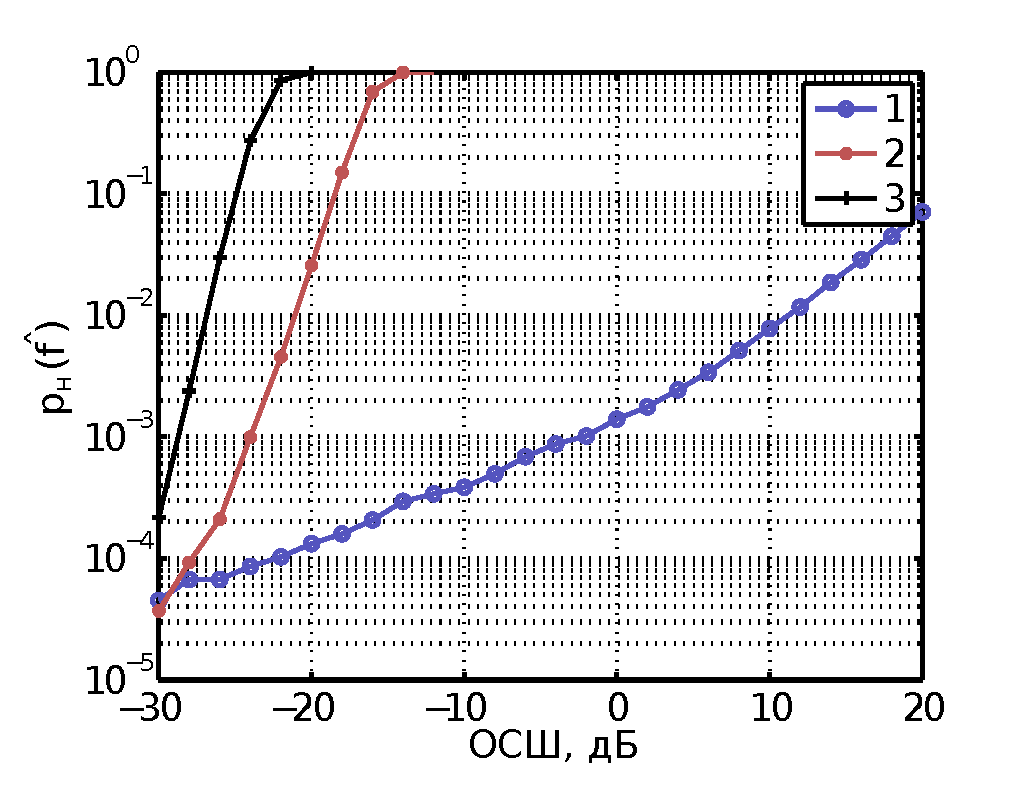
\includegraphics[width=1\linewidth]{ar_dma_probability.eps}}
	\caption{Вероятность оценки частоты удовлетворяющей допустимой входной расстройке}
	\label{pic:ar_dma_probability}
\end{figure}


